\documentclass[12pt,letterpaper]{article}
\usepackage{fullpage}
\usepackage[top=2cm, bottom=4.5cm, left=2.5cm, right=2.5cm]{geometry}
\usepackage{amsmath,amsthm,amsfonts,amssymb,amscd}
\usepackage{pythontex}
\usepackage{lastpage}
\usepackage{enumerate}
\usepackage{fancyhdr}
\usepackage{mathrsfs}
\usepackage{xcolor}
\usepackage{graphicx}
\usepackage{listings}
\usepackage{hyperref}
\usepackage{slashed}
\usepackage{subfigure}
\usepackage{subcaption}
\usepackage{graphicx,epstopdf}
\hypersetup{%
  colorlinks=true,
  linkcolor=blue,
  linkbordercolor={0 0 1}
}
 
\renewcommand\lstlistingname{Algorithm}
\renewcommand\lstlistlistingname{Algorithms}
\newcommand\norm[1]{\left\lVert#1\right\rVert}
\def\lstlistingautorefname{Alg.}

\lstdefinestyle{Python}{
    language        = Python,
    frame           = lines, 
    basicstyle      = \footnotesize,
    keywordstyle    = \color{blue},
    stringstyle     = \color{green},
    commentstyle    = \color{red}\ttfamily
}

\setlength{\parindent}{0.0in}
\setlength{\parskip}{0.05in}

% Edit these as appropriate
\newcommand\course{MAT162}
\newcommand\hwnumber{3}                  % <-- homework number
\newcommand\NetIDa{}           % <-- NetID of person #1
\newcommand\NetIDb{Gess Iraji}           % <-- NetID of person #2 (Comment this line out for problem sets)

\pagestyle{fancyplain}
\headheight 35pt
\lhead{\NetIDa}
\lhead{\NetIDa\\\NetIDb}                 % <-- Comment this line out for problem sets (make sure you are person #1)
\chead{\textbf{\Large Homework \hwnumber}}
\rhead{\course \\ \today}
\lfoot{}
\cfoot{}
\rfoot{\small\thepage}
\headsep 1.5em

\begin{document}

\section*{Problem 1}
\textbf{a)} 
Let $ F = I-2 \textbf{x} \mathbf{x^T}$ be a 3$\times$3 reflection matrix with $\textbf{x}$ a normalized 3 vector ($|x|=1$) and I the identity. We want to show that 
$$F^T F = F F^T = I.$$ In tensor notation (repeated indices denote summation), we can write:
$$F = \delta_{ij} - x_i x_j$$
First, due to the properties of the transpose, we know that
$$ F^T = (\delta_{ij} - 2 x_i x_j)^T = \delta_{ij}^T  - 2 (x_i x_j)^T =  \delta_{ij}  - 2 (x_j x_i)  $$
Now, we have
$$F^T F = (\delta_{ik}  - 2 (x_i x_k))(\delta_{kj}  - 2 (x_k x_j))  = \delta_{ij} -2(x_i x_j)-2(x_i x_j)+4 (x_i x_k)(x_k x_j)=I -4x_i x_j +4(x_i x_j) (x_k x_k) = I.$$
where the last step follows since $\sum x_k x_k = 1$ (x is normalized). Similarly, we can show that$ F F^T = I$. Thus, $F^T = F^{-1}$ as required.
\newline
\newline \textbf{b)} Let $\{x,y_2,y_3\}$ be an orthonormal basis for $\mathbb{R}^3$. We want to evaluate F\textbf{x}. Let 
$x =
\begin{bmatrix}
x_1 \\
x_2 \\
x_3
\end{bmatrix}
$
then

$$F = I - 2 x x^T =
\begin{bmatrix}
1-2x_1 x_1 & -2x_1 x_2 & -2x_1 x_3 \\
-2x_2 x_1 & 1-2x_2 x_2 & -2x_2 x_3 \\
-2x_3 x_1 & -2x_3 x_2 & 1-2x_3 x_3 
\end{bmatrix}
$$and
$$ F x = 
\begin{bmatrix}
1-2x_1 x_1 & -2x_1 x_2 & -2x_1 x_3 \\
-2x_2 x_1 & 1-2x_2 x_2 & -2x_2 x_3 \\
-2x_3 x_1 & -2x_3 x_2 & 1-2x_3 x_3 
\end{bmatrix}
\begin{bmatrix}
x_1 \\
x_2 \\
x_3
\end{bmatrix}  $$
$$ = \begin{bmatrix}
(x_1)(1-2x_1^2) -2x_1 x_2^2 -2x_1 x_3^2 \\
(x_1)(-2x_2 x_1) + (x_2)(1-2x_2^2 ) -2x_2 x_3^2  \\
-2x_3 x_1^2 -2x_3 x_2^2  (1-2x_3^2 ) (x_3)
\end{bmatrix}
 =\begin{bmatrix}
(x_1)(1-2(x_1^2+x_2^2+x_3^2) \\
(x_2)(-2(x_1^2 + x_2^2+x_3^2)+1)  \\
(-2(x_1^2+ x_2^2 + x_3^2)+1) (x_3)
\end{bmatrix}
  = \begin{bmatrix}
-x_1\\
-x_2  \\
-x_3
\end{bmatrix} = -x$$
In tensor notation:
$$ F_{ij}\mathbf{y}_{2,j} = (\delta_{ij} - 2 x_i x_j) y_{2,j} = (y_{2,i} - 2  x_j (x_i y_{2,i}))= y_{2,i}=y_2 $$
last result follows since x and $y_2$ are orthogonal. Very similarly, we have $ F y_3 =y_3$. 
\newline Thus, $x,y_2,y_3$ are eigenvectors of F, with eigenvalues -1,1,1 respectively.
\newline
\newline \textbf{c)} Let V be a 3$\times $3 matrix with columns x, $y_2$ and $y_3$, and D a diagonal matrix with diagonal entries -1,1, and 1, respectively. We can write the eigendecomposition of F as
$$ F = VDV^{-1} = \begin{bmatrix}
x_1 & y_{2,1} &  y_{3,1}\\
x_2 & y_{2,2}& y_{3,2} \\
x_3 &  y_{2,3} & y_{3,3}
\end{bmatrix} 
\begin{bmatrix}
-1 & 0 &  0\\
0 & 1 & 0\\
0 & 0 & 1
\end{bmatrix} 
\begin{bmatrix}
x_1 &x_2  &  x_3\\
y_{2,1} & y_{2,2}&  y_{2,3} \\
y_{3,1} &y_{3,2}  & y_{3,3}
\end{bmatrix}
$$  
Since the columns of V form an orthonormal basis of $\mathbb{R}^3$, then V is orthogonal, and $V^{-1}=V^T$
\newline 
\newline 
\textbf{d)}Since F is positive definite and symmetric, its singular value decomposition (SVD) is given by the eigendecomposition:
$$ F = U \Sigma V^T =VDV^{-1}$$
so that
$$ F V = U \Sigma $$
which gives us the following equations of $F v = \sigma u:$
\newline $ 1. F (-x) = (1) (x) $
\newline $ 2. F y_2 =  (1)y_2 $
\newline $3. F y_3 =(1) y_3  $
\newline We note that $\sigma$ has to be non-negative here.
\newline \newline \textbf{e)} The singular values are given above (1,1,1). The rank of F is given by the number of nonzero singular values. In this case, F has full rank (3). Since F is orthogonal, it has norm 1, and its inverse has norm 1, so $cond(F)=1$.
\newline
\newline \textbf{f)} Using the QR algorithm, after $\boxed{44 \text{ iterations}}$, we get $\{ -1,-1,0.8 \}$ as our eigenvalues. \textbf{But this is incorrect.} First, the given vector is not normalized correctly. Second, Since F is orthogonal, QR is not going to work.



\vspace{1cm}

\section*{Problem 2} In this problem we consider the integral of the function $f(x) = \frac{1}{\frac{5}{4}-\cos \theta}$ over two intervals, first $[0,\pi/3],$ and then $[0,2 \pi]$. By the residue theorem, we know that the first should result in $8\pi/9$ and the second one $8 \pi/3$. 
\newline To calculate this integral, I wrote a function that performs composite trapezoid integration on this specific function. It takes the number of intervals and endpoints as its inputs, and computes the integral along with the theoretical error bound. The equation below gives us the error bound:
\begin{equation}
    E = \frac{\pi h^2}{36} \norm{\dfrac{2\sin^2\left(x\right)}{\left(\frac{5}{4}-\cos\left(x\right)\right)^3}-\dfrac{\cos\left(x\right)}{\left(\frac{5}{4}-\cos\left(x\right)\right)^2}}_\infty .
\end{equation}
The x-dependent part of the above equation, is the second derivative of the integrant. It has one minimum of $-16$ within both of the above intervals at 0. So we can either separately compute the error bound by 
\begin{equation}
    E = \frac{4\pi h^2}{9} 
\end{equation}
or just look at the maximum of the absolute value of the second derivative for each set.
for both parts of the problem. The plots show the absolute error, which I calculated by
\begin{equation}
    E_{absolute} = |I_{trapezoid} - \frac{8 \pi}{9}|,
\end{equation}
compared to the error bound. As we can see in these log-log plots, the absolute error always stays below the error bound. 
\newline If we compare the line corresponding to the error bound with the absolute error, we can guess that the absolute error is proportional to $h^2$ for the first plot.

\begin{figure}[h]
    \centering
    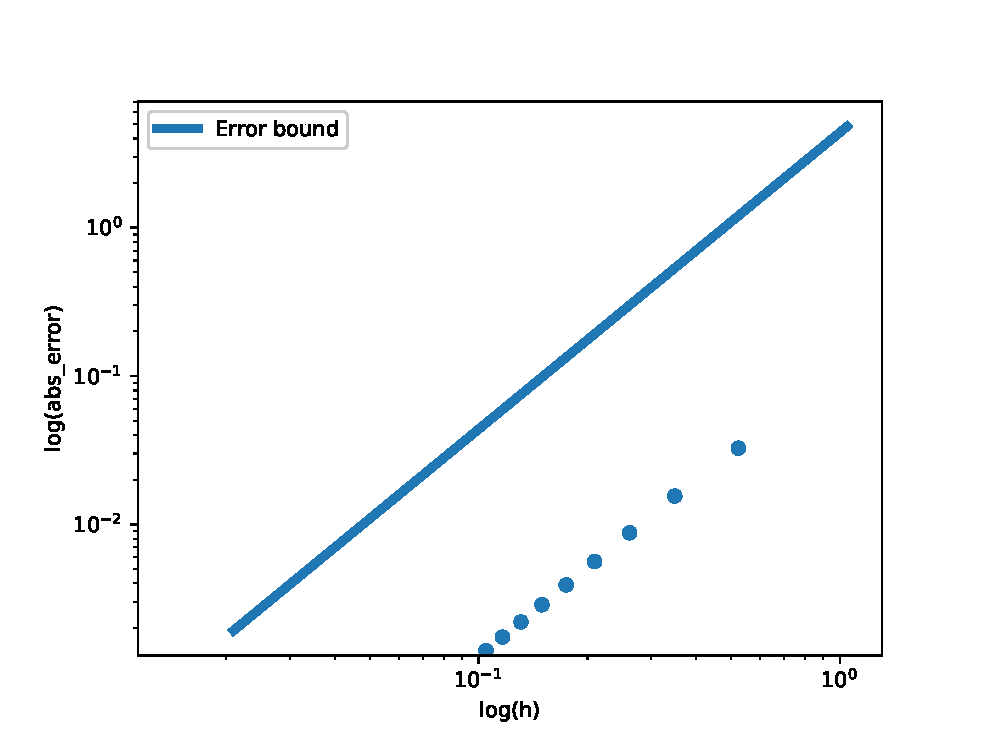
\includegraphics[width = 12cm]{Problem_2/hw3_2a.eps}
    \caption{Problem 2, part a. The error gets smaller as h gets smaller. Here, it scales as $h^2$} 
    \label{fig:2a}
\end{figure}

\begin{figure}[h]
    \centering
    \includegraphics[width = 12cm]{Problem_2/32a.eps}
    \caption{Problem 2, part a. Same plot, in case the scale looks strange with the scatter plot.} 
    \label{fig:2a}
\end{figure}


\begin{figure}[h]
    \centering
    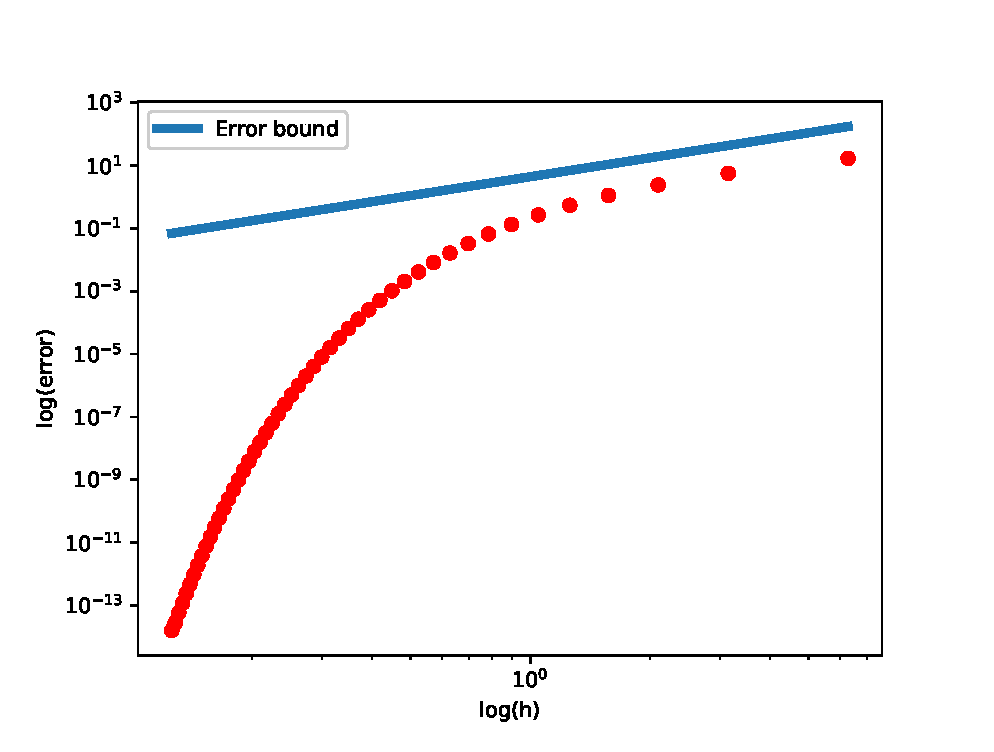
\includegraphics[width = 12cm]{Problem_2/hw3_2b.eps}
    \caption{Problem 2, part b. Again, the error gets smaller as h gets smaller. However, there is no general power law since the curve is not linear. We may be able to fit a line to this curve at different intervals, but not to the whole curve. }
    \label{fig:2b}
\end{figure}
\newline 
\textbf{c)} Consider $I = \int_0^{2\pi} \frac{1}{\frac{5}{4} - \cos \theta} d\theta$. We will choose the parametrization $z = e^{i \theta}$, and $dz = i e^{i \theta} d \theta = i z d \theta$. Then, by Euler's formula, we can write cosine as $$ cos \theta = \frac{e^{i \theta}+e^{-i \theta}}{2}.$$ So, we have
\begin{equation}
 I = \frac{2}{i}   \oint  \frac{dz}{z(\frac{5}{2} - (z+\frac{1}{z}))}
\end{equation}
The integrant has simple poles at 2 and $\frac{1}{2}$. The latter is inside our unit circle contour, where $$ f(z_0) = \frac{-2}{i(z_0 - 2)}  $$ so that $$ Res[f_0]_{z_0 = \frac{1}{2}} = \frac{2}{i(\frac{3}{2})} = \frac{4}{3i}. $$
Therefore, by Cauchy's residue theorem,
\begin{equation}
    I = \int_0^{2\pi} \frac{1}{\frac{5}{4} - \cos \theta} d\theta =\frac{2}{i}   \oint  \frac{dz}{z(\frac{5}{2} - (z+\frac{1}{z}))} = 2 \pi i(\frac{4}{3i})  = \frac{8 \pi}{3}
\end{equation}
as required.



\section*{Problem 3} \textbf{a)} Let $f:\mathbb{R} \xrightarrow{} \mathbb{R}$ be a function. We are interested in the integral of $f$ on $[a,b]$, $a,b \in \mathbb{R}$.  
\newline
\newline For this problem, I wrote a program that contains two functions: one that perform composite Simpsons rule on $m$ intervals, and one that tests the error against the tolerance level. We could follow the suggestion of the problem and write this differently, so that the first function only performs the $n = 1$ Simpsons integral on each interval, but after doing the algebra, that ends up being the same as the composite Simpsons rule: \begin{equation}
   Q_{2,h} = \frac{a-b}{6 m}\left(f(a)+4f(x_1)+2f(x_2)+...+4 f (x_{ 2m-1} )+ f (x_b )\right)
\end{equation}
We see that, excluding the endpoints, the terms with odd indices have coefficient 4 and those with even indices coefficient 2. For each term, depending on the residue of its index mod 2, I multiplied it by either 2 or 4.
\newline 
\newline
One thing that I had to be careful about was how I chose \textit{m} each round. Since each time I perform the integrals, I divide the intervals in half, all the number of intervals each round have the form of $2^n$. So first we have 2 intervals, then 4, then 8, and so on.
\newline \newline \textbf{b)}
The table shows my results for each of the integrals:
\begin{center}
 \begin{tabular}{||c c c c||} 
 \hline
 Integral & Q & Error ($|I_{n-1} - I_{n}|$)  & Number of Intervals \\ [0.5ex] 
 \hline\hline
 $\int_{-1}^1 |x|$ & 1.0000 & 0.0 & 4 \\ 
 \hline
 $\int_{-1}^2 |x|$ & 2.5000 & 0.0 & 2 \\
 \hline
  $\int_{0}^1 x^{3/4} \sin{(\frac{1}{x})}$ & 0.4070287 & 3.5810214680243035e-06 & 8192  \\ [1ex] 
 \hline
\end{tabular}
\end{center}

%[(0.9948915175883302, 1.9722716535386375e-05, 262), (2.4922779922779923, 2.9930262487543047e-05, 518), (0.40355896980274375, 4.386530552236145e-06, 166)]



\section*{Problem 4}

\textbf{a)} [No] Let $I = \int_{-1}^2 x^2 e^{-\lambda x^6} dx$, where $\lambda$ is much larger than 1. Although the function does not vary rapidly and $f(x) = x^6 $ has a global minimum in the interval $[-1,2]$, We can't apply Laplace's method. The second derivative is zero at this minimum and we cannot use the Taylor series expansion. 
\newline \newline \textbf{b)} We could approximate the integral in the following way:
\newline First, we use the substitution $u = x^3$ and $du = 3x^2 dx$ so that we arrive at a Gaussian integral:
\begin{equation}
    \int^8_{-1} \frac{e^{-\lambda u^2}}{3} du \sim  \int^\infty_{-\infty} \frac{e^{-\lambda u^2}}{3} du = \frac{\sqrt{\pi}}{3 \sqrt{\lambda}}
\end{equation}
Here, assuming $\lambda \gg 1$, as an approximation, we have expanded the limits of the integral to $(-\infty,\infty )$.
To compare the results with numerical approximation from Matlab, let's look at some plots:
\begin{figure}[h]
    \centering
    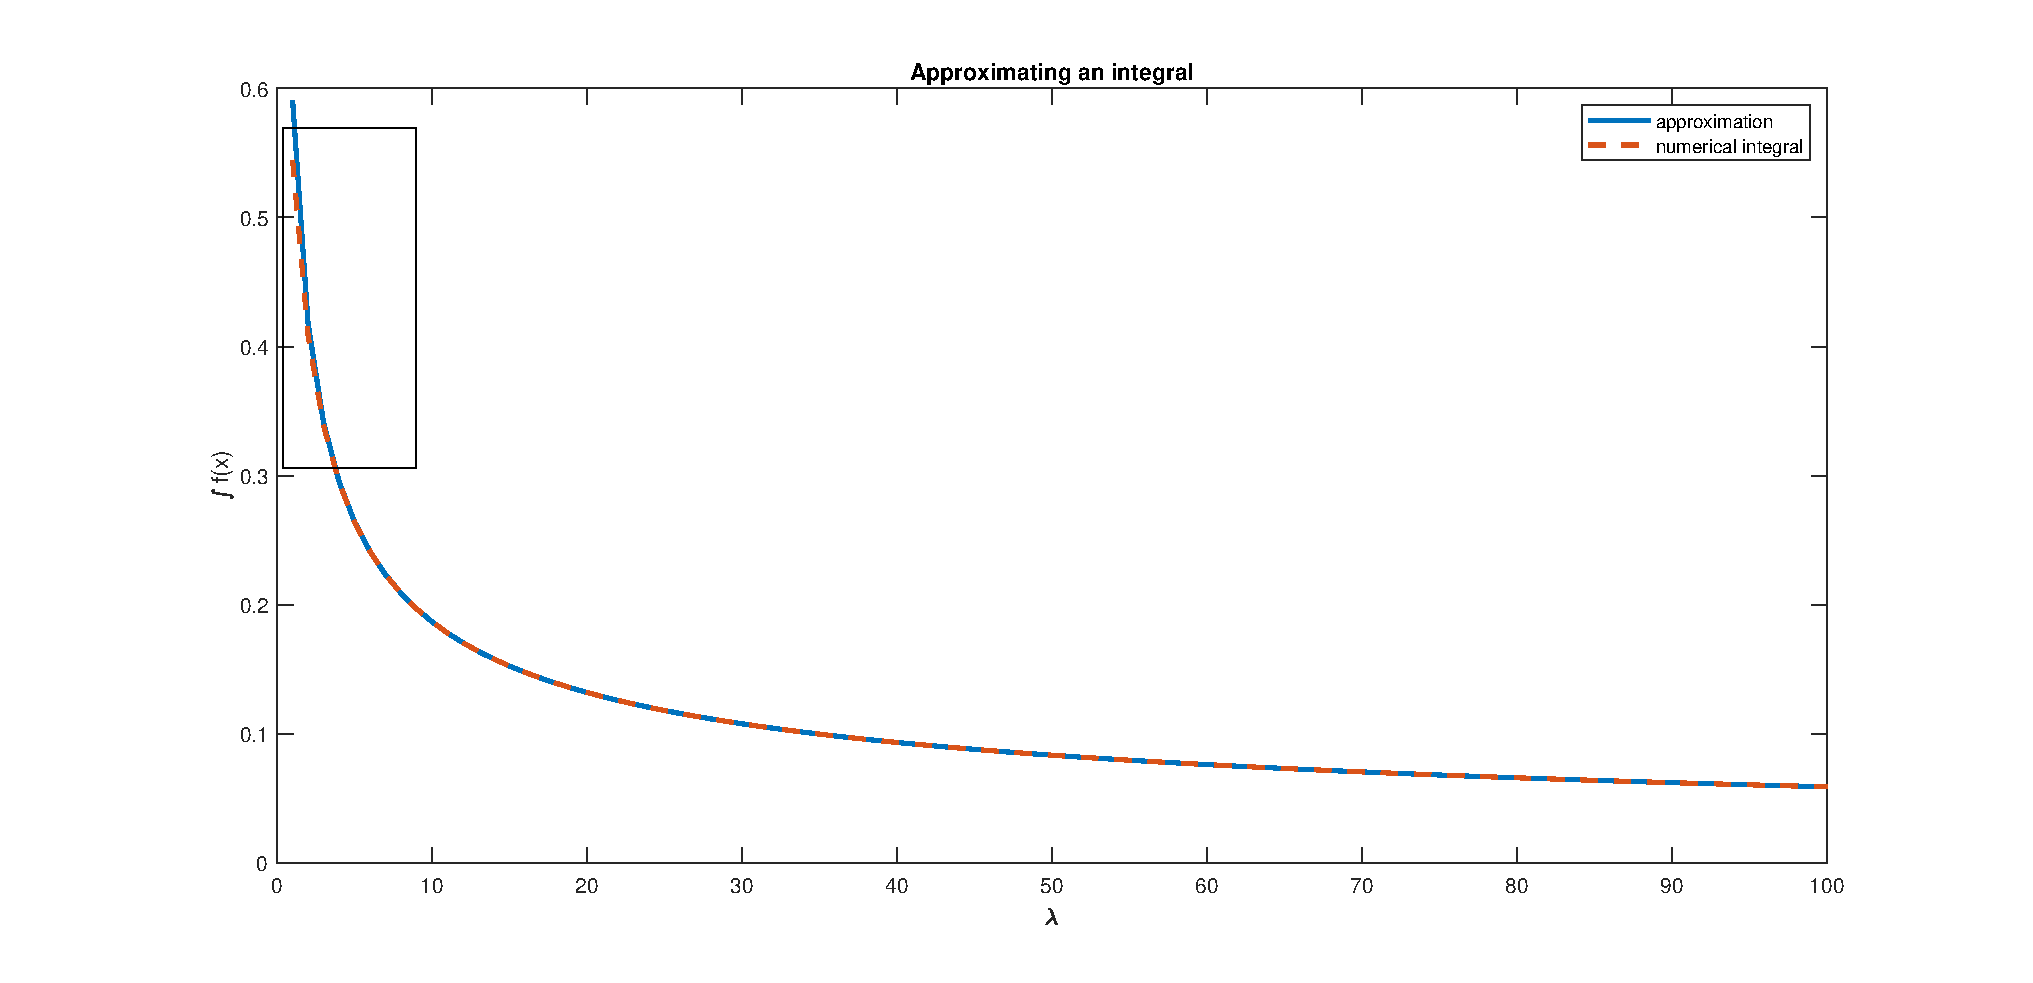
\includegraphics[height=9cm]{problem4/hw3_3_b.eps}
    \caption{This plot shows the numeric evaluation of the integral by Matlab compared to analytical approximation for $\lambda$ in the range $(1,100)$, with 1000 data points. We can see that the approximation matches more closely as we increase $\lambda$. The rectangle captures the points where the error is relatively greater compared to the other values. }
    \label{fig:fapp1}
\end{figure}
Figure \ref{fig:fapp1} shows the plot for the approximation of the first plot. Beyond a certain point (at about $\lambda = 15$), it is hard to tell how much of a better approximation we have by increasing $\lambda$. The plot of errors also reveals the same situation. After a point, the error drops drastically.
\begin{figure}[h]
    \centering
    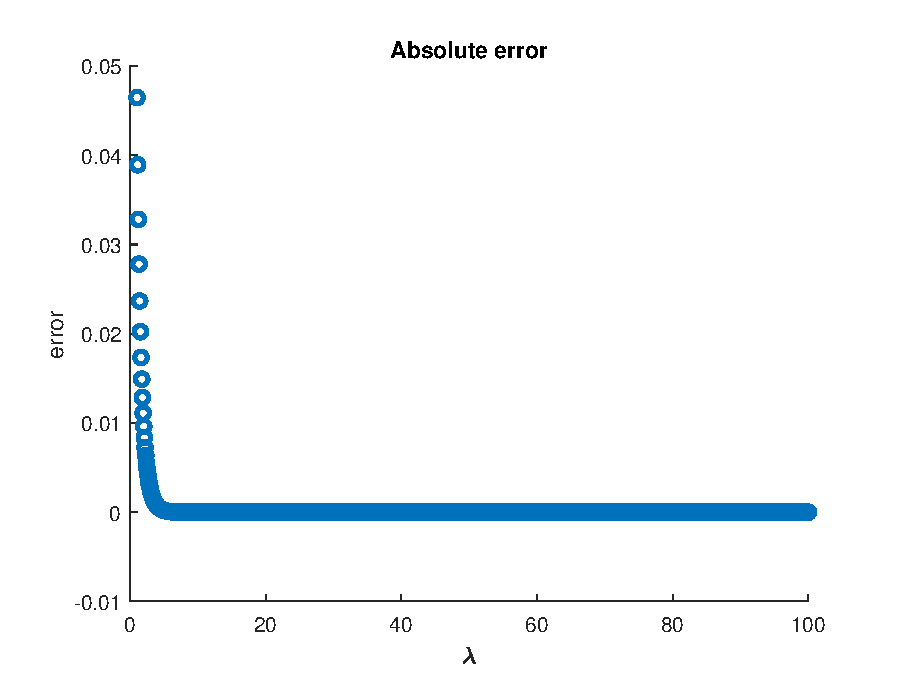
\includegraphics[height=9cm]{problem4/hw3_3_berror.eps}
    \caption{This plot shows the error for the first approximation. It gets extremely close to zero after we go past a critical $\lambda$. }
    \label{fig:ferror1}
\end{figure}
\vspace{1cm}
\newline \textbf{c)} Now, let $I_2 = \int_{-1}^2 (1+x^2) e^{-\lambda x^6} dx$. As we saw in class, we can use the Gamma function to approximate $\int_{-1}^2 e^{-\lambda x^6} dx$ and add our results from part b to complete the approximation. 
\newline Again, we start expanding the integration interval to  $(-\infty,\infty )$.
\begin{equation}
    I_2 \sim \int_{-\infty}^\infty e^{-\lambda x^6} dx = 2 \int_{0}^\infty e^{-\lambda x^6} dx 
\end{equation}
by using a substitution, in this case $u = \lambda x^6$ with $du = 6 \lambda x^5 dx = 6 \lambda (u/\lambda)^{5/6} dx$. Then we expand the interval:
\begin{equation}
   2 (\frac{1}{6 \lambda^{1/6}}) \int^\infty_{0} u^{\frac{1}{6}-1} {e^{- u}} du = (\frac{1}{3 \lambda^{1/6}}) \Gamma (\frac{1}{6}).
\end{equation}
Adding this to part b, we get
\begin{equation}
  I \sim \frac{1}{3} \left( \sqrt{\frac{\pi}{{\lambda}}} + \frac{\Gamma (\frac{1}{6})}{\lambda^{1/6}} \right).
\end{equation}
As we can see, the dominant term comes from the second approximation, $e^{-\lambda x^6}$. This is due to the fact that the majority of the area of the integral is densely located at $(-1,1)$. Since $|x|<1$ in this interval, the $x^2$ term make the overall $x^2 e^{-\lambda x^6}$ smaller compared to $ e^{-\lambda x^6}$.

\begin{figure}[h]
    \centering
    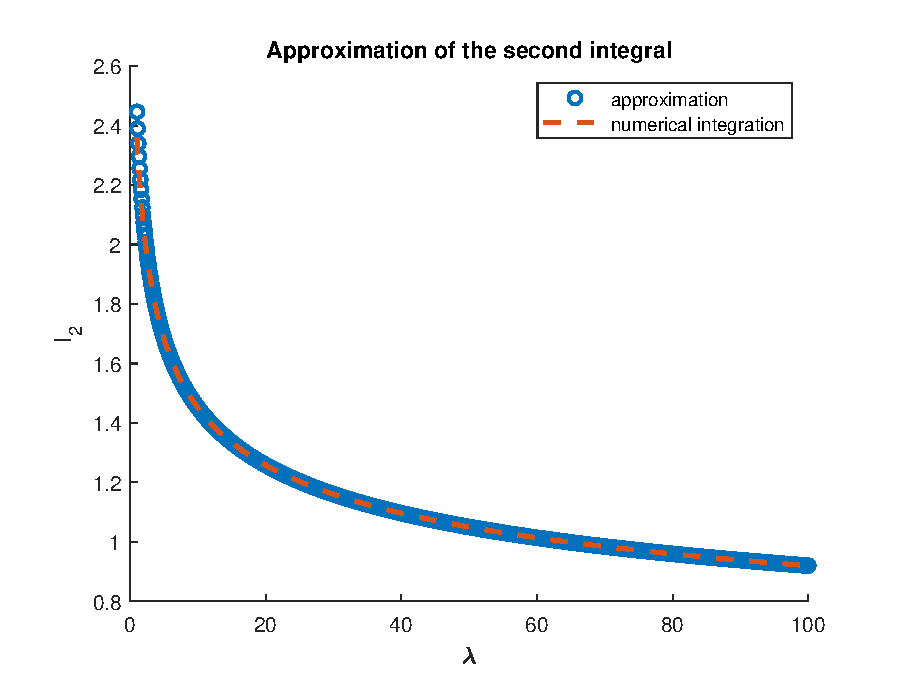
\includegraphics[height=9cm]{problem4/hw3_3_c.eps}
    \caption{(problem 4, part c)This plot shows the numeric evaluation of the second integral by Matlab compared to analytical approximation for $\lambda$ in the range $(1,100)$, with 1000 data points.  }
    \label{fig:fapp2}
\end{figure}


\begin{figure}[h]
    \centering
    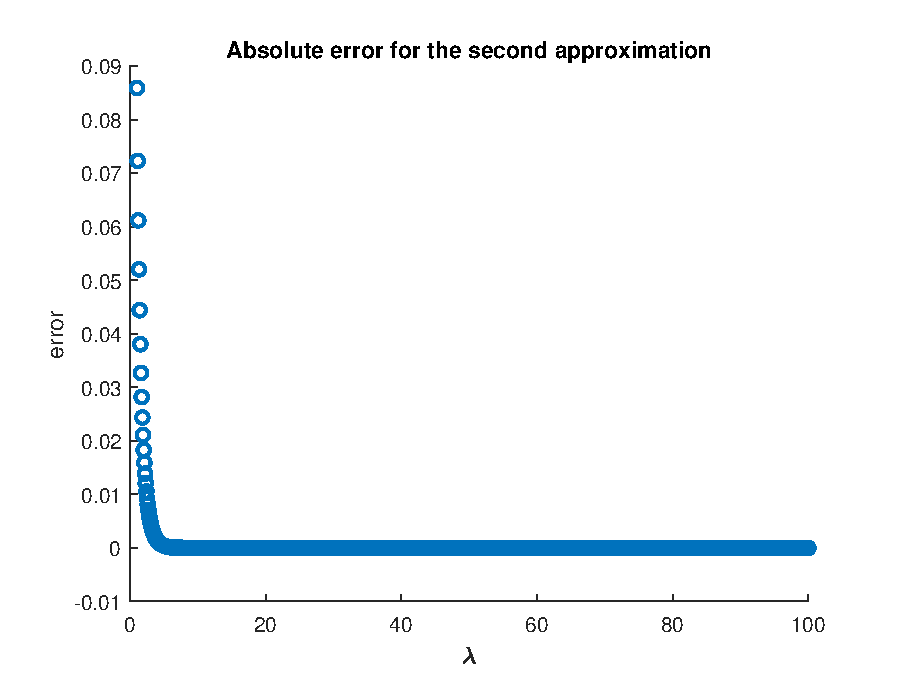
\includegraphics[height=9cm]{problem4/hw3_3_cerror.eps}
    \caption{(problem 4,c)This plot shows error when comparing the analytical approximation to the Matlab results. Again, the error gets smaller as we increase $\lambda$. }
    \label{fig:ferror2}
\end{figure}



\begin{figure}[h]
    \centering
    \includegraphics{problem4/hw3_4_b.jpg}
    \caption{(problem 4,b)The table shows exact and approximation values for the first integral. We see that as $\lambda$ gets larger, the error gets smaller. }
    \label{fig:ftab1}
\end{figure}

\begin{figure}[h]
    \centering
    \includegraphics{problem4/hw3_4_c.jpg}
    \caption{(problem 4,c)The table shows exact and approximation values for the second integral. Again, see that as $\lambda$ gets larger, the error gets smaller, to a point where we are limited by the finite precision of the machine. }
    \label{fig:ftab1}
\end{figure}


\end{document}


$F^T =
\begin{bmatrix}
1-2x_1 x_1 & -2x_1 x_2 & -2x_3 x_1 \\
-2x_1 x_2 & 1-2x_2 x_2 & -2x_3 x_2\\
-2x_3 x_1 & -2x_2 x_3 & 1-2x_3 x_3 
\end{bmatrix}
$ and we have
$$ F F^T = 
\begin{bmatrix}
(1-2x_1 x_1)^2+ 4x_1(x_2^2+x_3^2) & (-2x_1 x_2)(1-2x_1^2)+(1-2x_2^2)(-2x_1 x_2)+4x_1 x_2 x_3^2 & -2x_3 x_1 & 0 & \\
0 & 1 & \\
& & \\
\end{bmatrix}$$ 